\chapter{Opening angle of the ultrasound sensor}
\label{appendix:opening_angle}

The opening angle of the AR.Drone's ultrasound sensor is not documented.
A small experiment has been performed to determine the opening angle.

The AR.Drone was positioned at a fixed altitude of $79\small{cm}$ above a flat floor.
No obstacle was in range of the ultrasound sensor to make sure the measured altitude is the actual altitude of the AR.Drone.
The altitude measured by the ultrasound sensor was $75.2\small{cm}$, which equals a systematic error of $3.8\small{cm}$.
The AR.Drone's bottom camera was used to mark a point on the floor that is exactly below the center of the AR.Drone.
This point is equal to the center of ultrasound cone.
In order to measure the opening angle, floating objects were moved from outside the cone towards the cone.
The objects require a certain distance from the floor to achieve a distance short than the shortest distance between the sonar and the floor.
The minimal altitude of an object when assuming a maximum opening angle of $40$ degrees is:
\begin{equation}
a = 79\small{cm} - (cos(40\deg) \times 79\small{cm}) = 18.48\small{cm}
\end{equation}
Fluctuations in the altitude measurements indicate that the object is entering the cone.
The horizontal distance $d$ between the object and cone center (marked point) is the width of the cone and $h = 79\small{cm} - a$ is the height of the cone.
The angle $\alpha$ of the cone can be recovered with:
\begin{equation}
\alpha = tan^{-1}(d / h)
\end{equation}

The experiment was repeated $10$ times with different objects.
The average opening angle is $25.03^{\circ}$ with a standard deviation of $1.45^{\circ}$.





\chapter{Source code}
All source code is available at Google Code: \url{http://code.google.com/p/mscthesis-ndijkshoorn/}.
The recorded datasets, which are stored in YAML format, can be found at the downloads page: \url{http://code.google.com/p/mscthesis-ndijkshoorn/downloads/list}.

A research log can be found at \url{http://nickd.nl/wiki/thesis}.

\begin{figure}[htb]
\centering
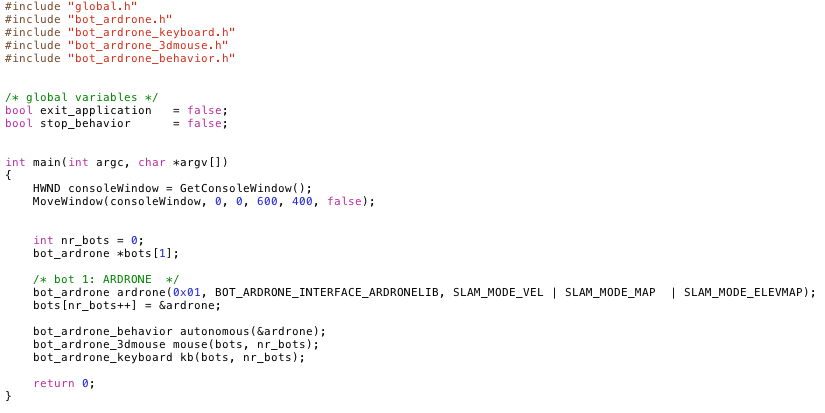
\includegraphics[width=\linewidth]{images/screenshot-code.png}
\caption{Source code of the application main file. This code initializes a robot instance and its controllers (autonomous behavior, keyboard and 3D mouse).}
\end{figure}